

\subsection{20.Если ошиблись в выборе Rk, то к чему это может привести?}
  Рассмотри на примере каскада с ОЭ
  \begin{center}
	\begin{figure}[h!]
		\center{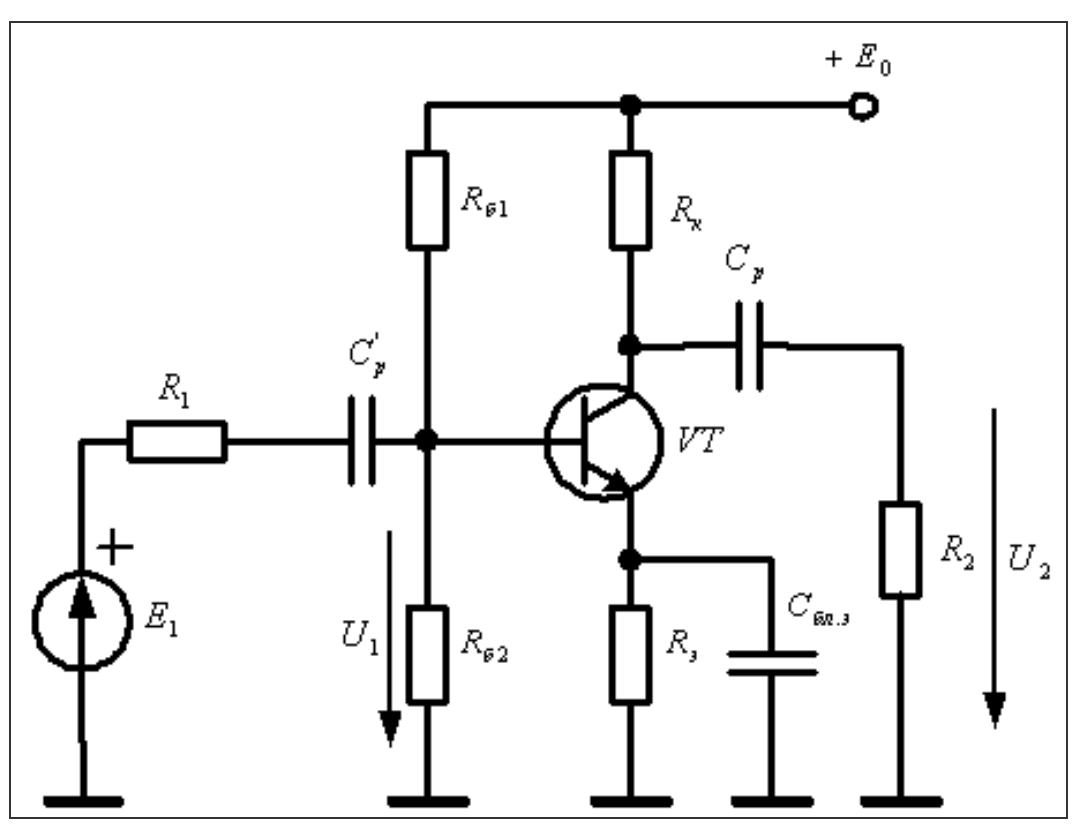
\includegraphics[scale=0.2]{oe.png}}
		\caption{каскад с ОЭ}	
		\label{OE}
	\end{figure}
\end{center}

Эквивалентная схема:

  \begin{center}
	\begin{figure}[h!]
		\center{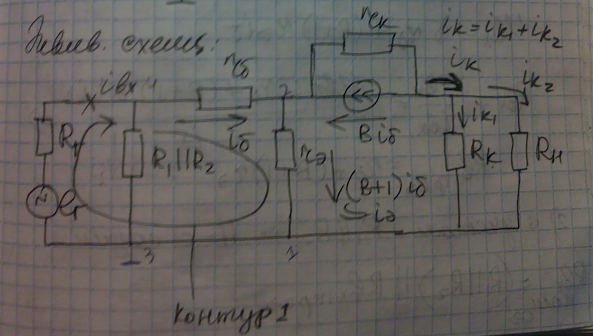
\includegraphics[scale=0.7]{oeekv.png}}
		\caption{эквивалентная схема каскада с ОЭ}	
		\label{EOE}
	\end{figure}
\end{center}

\ref{OEssil}

Резистор $R_k$ определяет коэффициент усиления по напряжению

При $R_g=0,R_H\rightarrow\infty   ,K_uoe=\frac{BR_k}{R_{vxtroe}}\Rightarrow$

Чем больше $R_k$, тем больше будет коэффициент передачи по напряжению.

Но согласно полной эквивалентной схемы(с $R_{kdif}$), $R_{kdif}$ ограничивает размер $R_{k}$, т.к. $R_k||r_{kdif}$

Также при больших значениях сопротивения $R_k$, весь потенциал $\varphi=E_k$ будет падать на нем и транзистор в результате не будет открываться.($I_{k0}$ будет ничтожно мал)

Рассмотрим схему:
  \begin{center}
	\begin{figure}[h!]
		\center{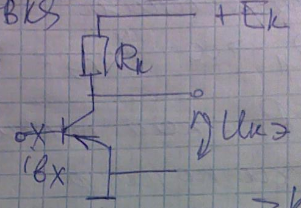
\includegraphics[scale=0.7]{20_sxem3.png}}
		\caption{каскад с ОЭ}	
		\label{20_1}
	\end{figure}
\end{center}

$R_k$ выбираем с учетом нужного коэффициента усиления, чем $R_k$ больше, тем больше и $K_u\Rightarrow$ меньший максимальной ток, протекающий через транзистор 
$$I_{max}=\frac{E_k}{R_k}$$

$R_k$ стоит || $R_H$, тогда
$$
i_{R_H}=i_k\frac{R_k}{R_k+R_H}б\,
$$
чем больше $R_k$, тем больше тока будет уходить в нагрузку

Коэффициент усиления по току так же зависит от значеня резистора $R_k$
$$
K_i=B\frac{R_k}{R_k+R_H}, 
$$
где чем больше $R_k$, тем больше $K_u$

Вывод: при очень больших значениях $R_k$ ток в транзисторе будет $\rightarrow0\Rightarrow$сигнал на выходе будет практически отсутствовать.

При малых значениях $R_k$ коэффициент училения по напряжению будет уменьшаться, но при этом ток в K будет расти$\Rightarrow$ при $R_k\rightarrow0,K_u\rightarrow0\Rightarrow$ на выходе сигнала опять таки не будет$\Rightarrow$ Для повышения коэффициента усиления, $R_k$ должно составлять несколько десятков кОМ, но при этом нужно увеличивать $E_k$(что затратно) и учитывать $R_kdif$. 